\documentclass{standalone}
\usepackage{tikz}
\usetikzlibrary{patterns, positioning}


\begin{document}
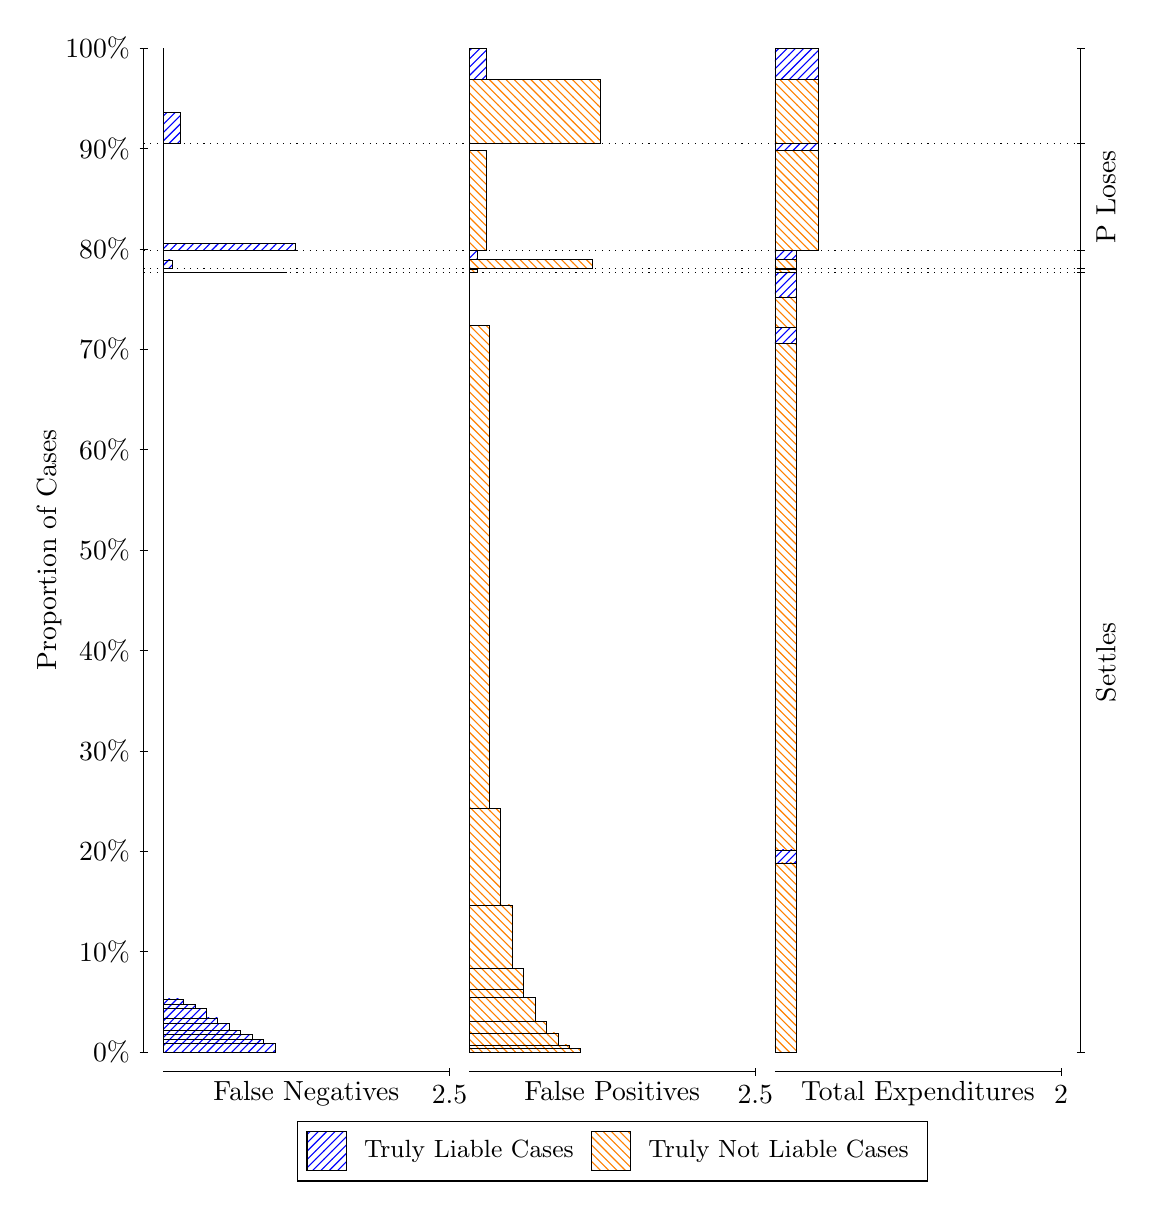
\begin{tikzpicture}
\draw[black, very thin] (1.5,1.75) -- (1.5,14.5);
\node[rotate=90, text=black, anchor=center] at (0.3, 8.125) {Proportion of Cases};
\draw[black, very thin] (1.45,1.75) -- (1.55,1.75);
\node[text=black, anchor=east] at (1.45, 1.75) {0\%};
\draw[black, very thin] (1.45,3.025) -- (1.55,3.025);
\node[text=black, anchor=east] at (1.45, 3.025) {10\%};
\draw[black, very thin] (1.45,4.3) -- (1.55,4.3);
\node[text=black, anchor=east] at (1.45, 4.3) {20\%};
\draw[black, very thin] (1.45,5.575) -- (1.55,5.575);
\node[text=black, anchor=east] at (1.45, 5.575) {30\%};
\draw[black, very thin] (1.45,6.85) -- (1.55,6.85);
\node[text=black, anchor=east] at (1.45, 6.85) {40\%};
\draw[black, very thin] (1.45,8.125) -- (1.55,8.125);
\node[text=black, anchor=east] at (1.45, 8.125) {50\%};
\draw[black, very thin] (1.45,9.4) -- (1.55,9.4);
\node[text=black, anchor=east] at (1.45, 9.4) {60\%};
\draw[black, very thin] (1.45,10.675) -- (1.55,10.675);
\node[text=black, anchor=east] at (1.45, 10.675) {70\%};
\draw[black, very thin] (1.45,11.95) -- (1.55,11.95);
\node[text=black, anchor=east] at (1.45, 11.95) {80\%};
\draw[black, very thin] (1.45,13.225) -- (1.55,13.225);
\node[text=black, anchor=east] at (1.45, 13.225) {90\%};
\draw[black, very thin] (1.45,14.5) -- (1.55,14.5);
\node[text=black, anchor=east] at (1.45, 14.5) {100\%};

\draw[black, very thin] (13.4,1.75) -- (13.4,14.5);
\draw[black, very thin] (13.35,1.75) -- (13.45,1.75);
\node[anchor=west] at (13.35, 1.75) {};
\draw[black, very thin] (13.35,11.651) -- (13.45,11.651);
\node[anchor=west] at (13.35, 11.651) {};
\draw[black, very thin] (13.35,11.697) -- (13.45,11.697);
\node[anchor=west] at (13.35, 11.697) {};
\draw[black, very thin] (13.35,11.929) -- (13.45,11.929);
\node[anchor=west] at (13.35, 11.929) {};
\draw[black, very thin] (13.35,13.289) -- (13.45,13.289);
\node[anchor=west] at (13.35, 13.289) {};
\draw[black, very thin] (13.35,14.5) -- (13.45,14.5);
\node[anchor=west] at (13.35, 14.5) {};

\draw[black, very thin, pattern color=blue, pattern=north east lines] (1.75,1.75) rectangle (3.167,1.8631);
\draw[black, very thin, pattern color=blue, pattern=north east lines] (1.75,1.8631) rectangle (3.0217,1.9082);
\draw[black, very thin, pattern color=blue, pattern=north east lines] (1.75,1.9082) rectangle (2.8763,1.9703);
\draw[black, very thin, pattern color=blue, pattern=north east lines] (1.75,1.9703) rectangle (2.731,2.0281);
\draw[black, very thin, pattern color=blue, pattern=north east lines] (1.75,2.0281) rectangle (2.5857,2.1138);
\draw[black, very thin, pattern color=blue, pattern=north east lines] (1.75,2.1138) rectangle (2.4403,2.1827);
\draw[black, very thin, pattern color=blue, pattern=north east lines] (1.75,2.1827) rectangle (2.295,2.3057);
\draw[black, very thin, pattern color=blue, pattern=north east lines] (1.75,2.3057) rectangle (2.1497,2.3567);
\draw[black, very thin, pattern color=blue, pattern=north east lines] (1.75,2.3567) rectangle (2.0043,2.4251);
\draw[black, very thin, pattern color=orange, pattern=north west lines] (1.75,2.4251) rectangle (1.75,11.651);
\draw[black, very thin, pattern color=blue, pattern=north east lines] (1.75,11.651) rectangle (3.3123,11.654);
\draw[black, very thin, pattern color=orange, pattern=north west lines] (1.75,11.654) rectangle (1.75,11.697);
\draw[black, very thin, pattern color=blue, pattern=north east lines] (1.75,11.697) rectangle (1.859,11.81);
\draw[black, very thin, pattern color=orange, pattern=north west lines] (1.75,11.81) rectangle (1.75,11.929);
\draw[black, very thin, pattern color=blue, pattern=north east lines] (1.75,11.929) rectangle (3.4213,12.018);
\draw[black, very thin, pattern color=orange, pattern=north west lines] (1.75,12.018) rectangle (1.75,13.289);
\draw[black, very thin, pattern color=blue, pattern=north east lines] (1.75,13.289) rectangle (1.968,13.683);
\draw[black, very thin, pattern color=orange, pattern=north west lines] (1.75,13.683) rectangle (1.75,14.5);
\draw[black, very thin, pattern color=orange, pattern=north west lines] (5.6333,1.75) rectangle (7.0503,1.7989);
\draw[black, very thin, pattern color=orange, pattern=north west lines] (5.6333,1.7989) rectangle (6.905,1.8409);
\draw[black, very thin, pattern color=orange, pattern=north west lines] (5.6333,1.8409) rectangle (6.7597,1.9914);
\draw[black, very thin, pattern color=orange, pattern=north west lines] (5.6333,1.9914) rectangle (6.6143,2.1382);
\draw[black, very thin, pattern color=orange, pattern=north west lines] (5.6333,2.1382) rectangle (6.469,2.4442);
\draw[black, very thin, pattern color=orange, pattern=north west lines] (5.6333,2.4442) rectangle (6.3237,2.5468);
\draw[black, very thin, pattern color=orange, pattern=north west lines] (5.6333,2.5468) rectangle (6.3237,2.8103);
\draw[black, very thin, pattern color=orange, pattern=north west lines] (5.6333,2.8103) rectangle (6.1783,3.6188);
\draw[black, very thin, pattern color=orange, pattern=north west lines] (5.6333,3.6188) rectangle (6.033,4.8448);
\draw[black, very thin, pattern color=orange, pattern=north west lines] (5.6333,4.8448) rectangle (5.8877,10.976);
\draw[black, very thin, pattern color=blue, pattern=north east lines] (5.6333,10.976) rectangle (5.6333,11.651);
\draw[black, very thin, pattern color=orange, pattern=north west lines] (5.6333,11.651) rectangle (5.7423,11.694);
\draw[black, very thin, pattern color=blue, pattern=north east lines] (5.6333,11.694) rectangle (5.6333,11.697);
\draw[black, very thin, pattern color=orange, pattern=north west lines] (5.6333,11.697) rectangle (7.1957,11.815);
\draw[black, very thin, pattern color=blue, pattern=north east lines] (5.6333,11.815) rectangle (5.7423,11.929);
\draw[black, very thin, pattern color=orange, pattern=north west lines] (5.6333,11.929) rectangle (5.8513,13.199);
\draw[black, very thin, pattern color=blue, pattern=north east lines] (5.6333,13.199) rectangle (5.6333,13.289);
\draw[black, very thin, pattern color=orange, pattern=north west lines] (5.6333,13.289) rectangle (7.3047,14.106);
\draw[black, very thin, pattern color=blue, pattern=north east lines] (5.6333,14.106) rectangle (5.8513,14.5);
\draw[black, very thin, pattern color=orange, pattern=north west lines] (9.5167,1.75) rectangle (9.7892,4.1505);
\draw[black, very thin, pattern color=blue, pattern=north east lines] (9.5167,4.1505) rectangle (9.7892,4.3156);
\draw[black, very thin, pattern color=orange, pattern=north west lines] (9.5167,4.3156) rectangle (9.7892,10.753);
\draw[black, very thin, pattern color=blue, pattern=north east lines] (9.5167,10.753) rectangle (9.7892,10.952);
\draw[black, very thin, pattern color=orange, pattern=north west lines] (9.5167,10.952) rectangle (9.7892,11.34);
\draw[black, very thin, pattern color=blue, pattern=north east lines] (9.5167,11.34) rectangle (9.7892,11.651);
\draw[black, very thin, pattern color=orange, pattern=north west lines] (9.5167,11.651) rectangle (9.7892,11.694);
\draw[black, very thin, pattern color=blue, pattern=north east lines] (9.5167,11.694) rectangle (9.7892,11.697);
\draw[black, very thin, pattern color=orange, pattern=north west lines] (9.5167,11.697) rectangle (9.7892,11.815);
\draw[black, very thin, pattern color=blue, pattern=north east lines] (9.5167,11.815) rectangle (9.7892,11.929);
\draw[black, very thin, pattern color=orange, pattern=north west lines] (9.5167,11.929) rectangle (10.062,13.199);
\draw[black, very thin, pattern color=blue, pattern=north east lines] (9.5167,13.199) rectangle (10.062,13.289);
\draw[black, very thin, pattern color=orange, pattern=north west lines] (9.5167,13.289) rectangle (10.062,14.106);
\draw[black, very thin, pattern color=blue, pattern=north east lines] (9.5167,14.106) rectangle (10.062,14.5);
\draw[black, dotted] (1.5,11.651) -- (13.4,11.651);
\draw[black, dotted] (1.5,11.697) -- (13.4,11.697);
\draw[black, dotted] (1.5,11.929) -- (13.4,11.929);
\draw[black, dotted] (1.5,13.289) -- (13.4,13.289);
\draw[black, very thin] (1.75,1.5) -- (5.3833,1.5);
\node[text=black, anchor=north] at (3.5667, 1.5) {False Negatives};
\draw[black, very thin] (5.3833,1.45) -- (5.3833,1.55);
\node[text=black, anchor=north] at (5.3833, 1.45) {2.5};

\draw[black, very thin] (5.6333,1.5) -- (9.2667,1.5);
\node[text=black, anchor=north] at (7.45, 1.5) {False Positives};
\draw[black, very thin] (9.2667,1.45) -- (9.2667,1.55);
\node[text=black, anchor=north] at (9.2667, 1.45) {2.5};

\draw[black, very thin] (9.5167,1.5) -- (13.15,1.5);
\node[text=black, anchor=north] at (11.333, 1.5) {Total Expenditures};
\draw[black, very thin] (13.15,1.45) -- (13.15,1.55);
\node[text=black, anchor=north] at (13.15, 1.45) {2};

\node[text=black, centered, rotate=90] at (13.72, 6.7005) {Settles};


\node[text=black, centered, rotate=90] at (13.72, 12.609) {P Loses};


\draw (7.449999999999999,1.5) node[draw=none] (baseCoordinate) {};
\begin{scope}[align=center]
        \matrix[scale=0.5, draw=black, below=0.5cm of baseCoordinate, nodes={draw}, column sep=0.1cm]{
            \node[rectangle, draw, minimum width=0.5cm, minimum height=0.5cm, pattern color=blue, pattern=north east lines] {}; &
            \node[draw=none, font=\small, text=black] (B) {Truly Liable Cases}; &
            \node[rectangle, draw, minimum width=0.5cm, minimum height=0.5cm, pattern color=orange, pattern=north west lines] {}; &
            \node[draw=none, font=\small, text=black] (B) {Truly Not Liable Cases}; \\
            };
\end{scope}

\end{tikzpicture}
\end{document}